\documentclass[tikz,border=10pt]{standalone}
\begin{document}
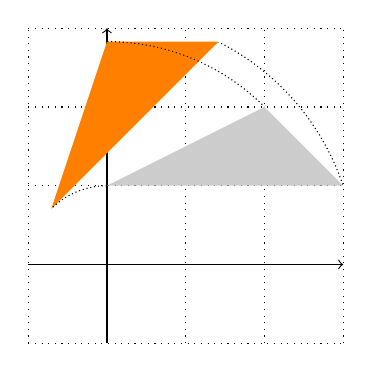
\begin{tikzpicture}
  % grid and coordinate axes:
  \draw[thin,dotted] (-1,-1) grid (3,3);
  \draw[->] (-1,0) -- (3,0);
  \draw[->] (0,-1) -- (0,3);
  % original triangle:
  \fill[gray!40] (0,1) -- (3,1) -- (2,2) --cycle;
  % rotated triangle:
  \fill[orange, rotate=45] (0,1) -- (3,1) -- (2,2) --cycle;
  % clipped circles to show the rotation:
  \begin{scope}
    \clip (0,1) rectangle (3,2.82);
    \draw[densely dotted] circle(3.16);
  \end{scope}
  \begin{scope}
    \clip (0,3) rectangle (2,2);
    \draw[densely dotted] circle(2.83);
  \end{scope}
  \begin{scope}
    \clip (-0.7,0.6) rectangle (0,1);
    \draw[densely dotted] circle(1);
  \end{scope}
\end{tikzpicture}
\end{document}
